\chapter{Warna dan Absorbans}\label{ch:g11:absorbance}

Sebotol minuman olahraga berpendar biru terang di atas bangku sebuah
pusat kebugaran. Warnanya berasal dari zat warna yang terlarut di
dalamnya, beberapa miligram dalam satu liter penuh: terlalu sedikit untuk
ditimbang, dan terlalu sedikit untuk terlihat sebagai padatan. Namun
laboratorium pangan harus memeriksa jumlah itu, karena zat warna hanya
boleh ditambahkan dalam batas tertentu. Warna itu sendirilah kuncinya.
Makin banyak zat warna yang dikandung sebuah larutan, makin banyak
cahaya yang diserapnya; alat yang mengukur berapa banyak cahaya yang
diserap sebuah larutan sebenarnya mengukur konsentrasi.

\begin{recall}
\omterm{def:g10:concentration-and-dilution:mass-concentration}{Konsentrasi massa} dan \omterm{def:g10:concentration-and-dilution:molar-concentration}{konsentrasi molar} sebuah larutan; mengencerkan
\omterm{def:g10:concentration-and-dilution:dilution}{larutan induk}; \omterm{def:g10:concentration-and-dilution:standard}{skala kalibrasi} larutan-larutan standar yang dibandingkan
dengan larutan yang tidak diketahui
(\cref{ch:g10:concentration-and-dilution}).
\end{recall}

\begin{omfigure}
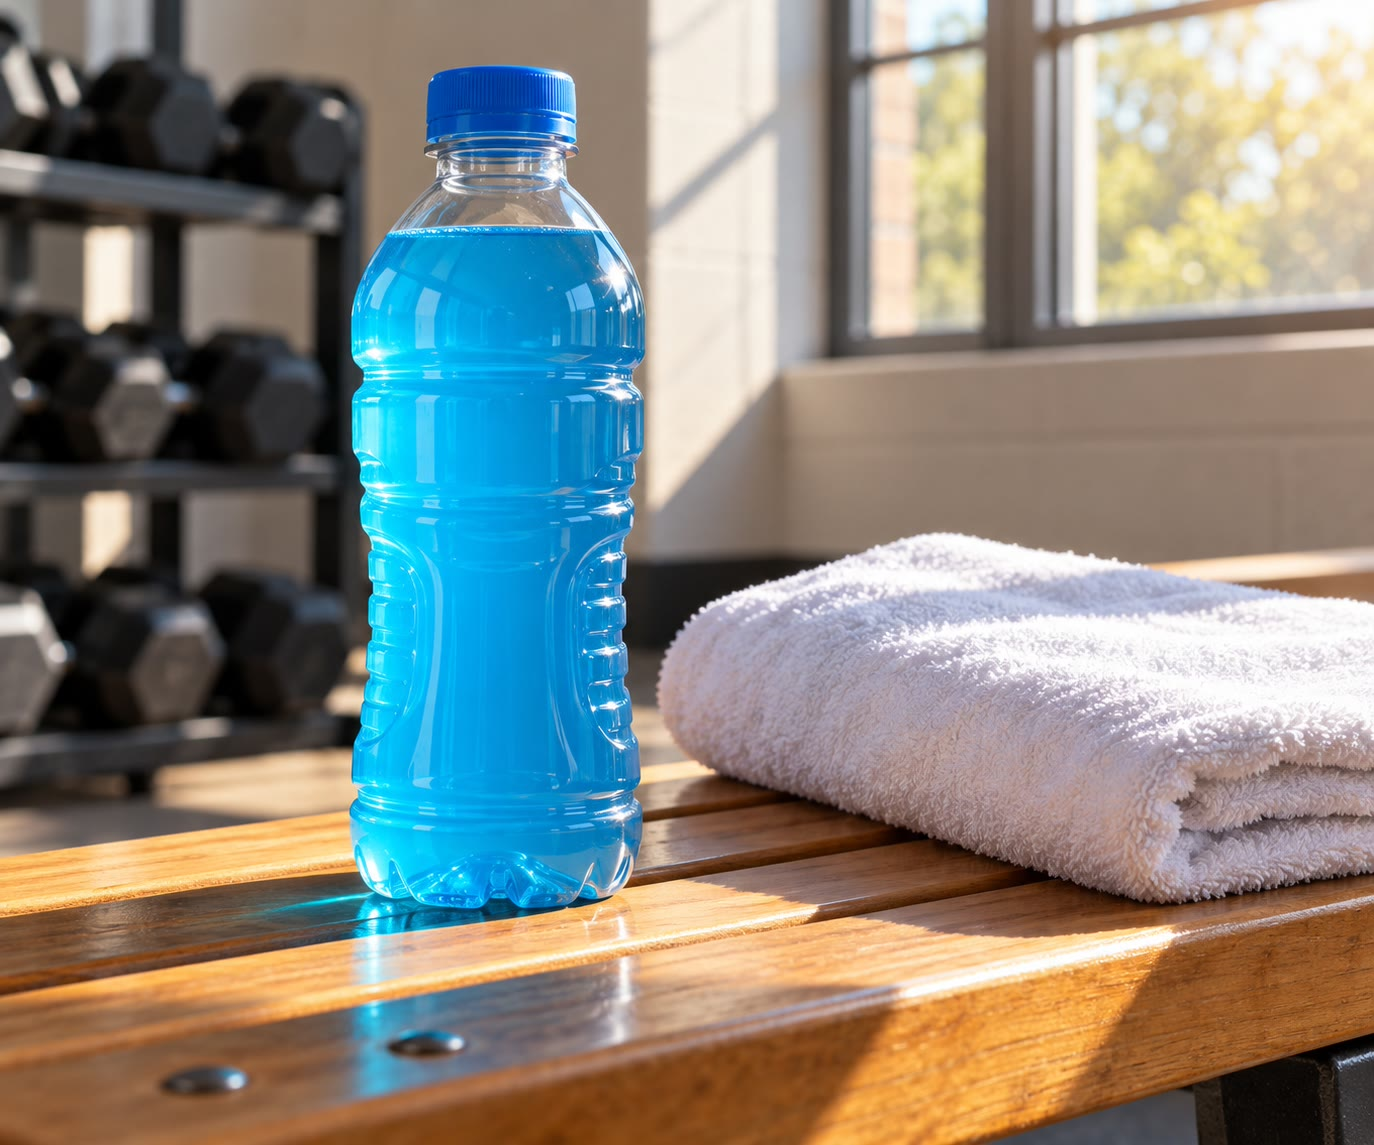
\includegraphics[width=0.5\linewidth]{images/book1/ai/g11-sports-drink.jpg}

{\small Minuman biru: warnanya berasal dari beberapa miligram zat warna
per liter.}
\end{omfigure}

\section{Warna sebuah larutan}

Cahaya putih, seperti cahaya siang hari, adalah \omterm{def:g6:pure-substances-and-mixtures:mixture}{campuran} semua warna
pelangi. Setiap warna berkaitan dengan sebuah panjang gelombang, dari
sekitar \qty{400}{nm} untuk ungu sampai sekitar \qty{750}{nm} untuk
merah; buku fisika menjelaskan apa itu panjang gelombang, dan di sini
panjang gelombang hanya menjadi label sebuah warna. Larutan berwarna
menyerap sebagian cahaya yang melewatinya, ada warna yang jauh lebih
banyak diserap daripada yang lain; mata melihat warna-warna yang lolos.

\begin{definition}[Warna komplementer]\label{def:g11:absorbance:complementary}
Dua warna disebut \emph{warna komplementer}\index{warna komplementer}
jika \omterm{def:g6:pure-substances-and-mixtures:mixture}{campuran} keduanya menghasilkan cahaya putih. Pada roda warna,
warna-warna komplementer saling berhadapan.
\end{definition}

\begin{omfigure}
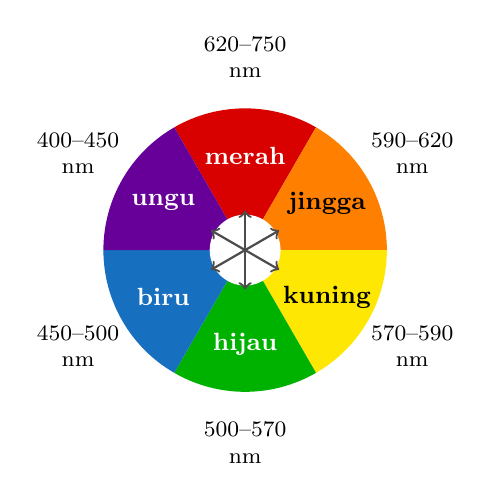
\begin{tikzpicture}[font=\small]
  \foreach \a/\c/\n/\w/\t in {90/red!85!black/merah/{620--750}/white,
      30/orange/jingga/{590--620}/black, -30/yellow!90!orange/kuning/{570--590}/black,
      -90/green!70!black/hijau/{500--570}/white, -150/cyan!50!blue/biru/{450--500}/white,
      150/violet!80!blue/ungu/{400--450}/white} {
    \fill[\c] (0,0) -- (\a-30:1.8) arc[start angle=\a-30, end angle=\a+30,
      radius=1.8] -- cycle;
    \node[text=\t, font=\small\bfseries] at (\a:1.2) {\n};
    \node[font=\footnotesize, align=center] at (\a:2.45) {\w\\ nm};
  }
  \fill[white] (0,0) circle (0.45);
  \draw[<->, thick, black!70] (90:0.5) -- (-90:0.5);
  \draw[<->, thick, black!70] (30:0.5) -- (-150:0.5);
  \draw[<->, thick, black!70] (-30:0.5) -- (150:0.5);
\end{tikzpicture}

{\small Roda warna, dengan panjang gelombang perkiraan. Warna-warna
komplementer saling berhadapan: merah dan hijau, jingga dan biru, kuning
dan ungu.}
\end{omfigure}

\begin{proposition}[Warna yang terlihat]\label{prop:g11:absorbance:colour-seen}
Larutan yang terutama menyerap satu warna dari cahaya putih tampak
berwarna komplementernya.
\end{proposition}

\begin{proof}
Diterima tanpa bukti: cahaya yang lolos adalah cahaya putih dikurangi
warna yang diserap, dan mata melihat sisa itu sebagai \omterm{def:g11:absorbance:complementary}{warna
komplementernya}.
\end{proof}

\begin{example}[Dua zat warna makanan]\label{ex:g11:absorbance:dyes}
% ledger: lmax:E133, lmax:E102
Zat warna biru dalam minuman olahraga itu, yang dikenal sebagai
biru berlian (E133), terutama menyerap cahaya jingga kemerahan, sekitar
\qty{629}{nm}: zat itu tampak biru. Zat warna kuning tartrazin (E102)
terutama menyerap cahaya biru keunguan, sekitar \qty{427}{nm}: zat itu
tampak kuning. Minuman hijau biasanya mengandung keduanya.
\end{example}

\section{Spektrum serapan}

\begin{definition}[Spektrum serapan]\label{def:g11:absorbance:spectrum}
Yang disebut \emph{spektrum serapan}\index{spektrum serapan} sebuah
larutan adalah grafik cahaya yang diserapnya (\omterm{def:g11:absorbance:absorbance}{absorbansnya}, yang
didefinisikan pada subbab berikutnya) terhadap panjang gelombang.
Panjang gelombang tempat serapannya paling besar ditulis
$\lambda_{\max}$.
\end{definition}

\begin{omfigure}
\begin{tikzpicture}
\begin{axis}[width=0.85\linewidth, height=6cm, xmin=380, xmax=750,
    ymin=0, ymax=0.95, xlabel={panjang gelombang $\lambda$ (\si{nm})},
    ylabel={absorbans $A$}, axis lines*=left, ymajorgrids,
    grid style={gray!20}, tick label style={font=\small},
    label style={font=\small}, xtick={400,450,500,550,600,650,700,750},
    ]
  % ledger: lmax:E133, abs:E133, lmax:E102, abs:E102 (band shapes synthetic)
  \addplot[very thick, cyan!60!blue] table[x=lambda, y=E133]
    {figdata/out/grade-11-absorbance-a.dat};
  \addplot[very thick, orange!85!yellow] table[x=lambda, y=E102]
    {figdata/out/grade-11-absorbance-a.dat};
  \node[font=\small, align=left, anchor=west, text=cyan!60!blue!80!black]
    at (axis cs:668,0.62) {zat warna\\ biru E133,\\ \qty{5.0}{mg/L}};
  \node[font=\small, align=left, anchor=west, text=orange!80!black]
    at (axis cs:470,0.66) {zat warna kuning E102,\\ \qty{15}{mg/L}};
  \addplot[dashed, black!50] coordinates {(629,0) (629,0.82)};
  \addplot[dashed, black!50] coordinates {(427,0) (427,0.795)};
  \node[font=\small, anchor=south] at (axis cs:629,0.83) {\qty{629}{nm}};
  \node[font=\small, anchor=south] at (axis cs:427,0.81) {\qty{427}{nm}};
\end{axis}
\end{tikzpicture}

{\small \omterm{def:g11:absorbance:spectrum}{Spektrum serapan} kedua zat warna dalam air, dalam kuvet setebal
\qty{1}{cm}. Bentuk pitanya digambar dari sebuah model sederhana;
letak puncak-puncaknya dan tingginya sesuai dengan spesifikasi kedua
zat warna itu.}
\end{omfigure}

\begin{remark}[Membaca spektrum]\label{rem:g11:absorbance:reading}
Zat warna biru hampir tidak menyerap apa pun di bawah \qty{520}{nm}:
cahaya biru dan ungu lolos, dan larutannya tampak biru. Zat warna kuning
hampir tidak menyerap apa pun di atas \qty{520}{nm}: cahaya hijau,
kuning, jingga, dan merah lolos, dan mata melihat kuning. Pada
\qty{629}{nm}, hanya zat warna biru yang menyerap; pada \qty{427}{nm},
hampir hanya zat warna kuning.
\end{remark}

\section{Absorbans dan spektrofotometer}

\begin{definition}[Absorbans]\label{def:g11:absorbance:absorbance}
Yang disebut \emph{absorbans}\index{absorbans} $A$ sebuah larutan, pada
panjang gelombang yang dipilih, adalah bilangan yang ditampilkan
spektrofotometer, yang mengukur berapa banyak cahaya dengan panjang
gelombang itu yang diserap larutan. Absorbans tidak bersatuan; nilainya
nol untuk \omterm{def:g6:solutions-and-solubility:solute}{pelarut} murni, dan makin besar jika makin banyak cahaya yang
diserap larutan.
\end{definition}

\begin{omfigure}
\begin{tikzpicture}[font=\small]
  % lamp
  \shade[ball color=yellow!40] (0,0.6) circle (0.32);
  \foreach \a in {0,45,90,135,180,225,270,315} \draw[yellow!60!orange, thick] (\a:0.4) ++(0,0.6) -- ++(\a:0.18);
  \node[anchor=north] at (0,-0.25) {lampu};
  \draw[black!60, thick] (0.8,0.6) -- (1.75,0.6);
  % prism
  \fill[cyan!10, draw=black!60] (1.75,0.15) -- (2.55,0.15) -- (2.15,1.15) -- cycle;
  \node[anchor=north] at (2.15,-0.25) {prisma};
  \foreach \c/\d in {violet/0.35, blue/0.22, green!70!black/0.08, yellow!90!orange/-0.06,
      orange/-0.2, red/-0.34}
    \draw[\c, thick] (2.45,0.6) -- (3.45,{0.6+\d});
  % slit
  \fill[black!70] (3.5,0.92) rectangle (3.6,1.4);
  \fill[black!70] (3.5,-0.2) rectangle (3.6,0.52);
  \node[anchor=north] at (3.55,-0.25) {celah};
  \draw[orange, very thick] (3.6,0.6) -- (4.75,0.6);
  % cuvette
  \pic (cv) at (5,0) {cuvette={0.75}{cyan!50!blue!45}};
  \node[anchor=north] at (5,-0.25) {kuvet};
  \draw[orange!60, thick] (5.3,0.6) -- (6.3,0.6);
  % detector and display
  \fill[black!15, draw=black!60] (6.3,0.2) rectangle (6.9,1.0);
  \node[anchor=north] at (6.6,-0.25) {detektor};
  \draw[black!60] (6.9,0.6) -- (7.4,0.6);
  \fill[black!80, draw=black] (7.4,0.25) rectangle (9.4,0.95);
  \node[green!70!white, font=\footnotesize\ttfamily] at (8.4,0.6) {A = 0.590};
  \node[anchor=north] at (8.4,-0.25) {layar};
\end{tikzpicture}

{\small Prinsip kerja spektrofotometer. Prisma menguraikan cahaya putih
menjadi warna-warnanya; celah hanya meloloskan satu panjang gelombang,
yang dipilih pemakai; detektor membandingkan cahaya yang keluar dari
kuvet dengan cahaya yang masuk ke dalamnya, dan layar menampilkan
\omterm{def:g11:absorbance:absorbance}{absorbansnya}.}
\end{omfigure}

\begin{remark}[Asal bilangan itu]\label{rem:g11:absorbance:log}
\omterm{def:g11:absorbance:absorbance}{Absorbans} dihitung oleh alat itu dari intensitas cahaya yang masuk ke
dalam larutan dan yang keluar darinya, dengan sebuah fungsi matematika
yang dipelajari pada tahun terakhir sekolah, yaitu logaritma. Salah satu
buku universitas memberikan rumusnya; di sini, \omterm{def:g11:absorbance:absorbance}{absorbans} hanyalah angka
yang dibaca alat itu.
\end{remark}

\begin{inthelab}[Menolkan spektrofotometer]
Kuvet, \omterm{def:g6:solutions-and-solubility:solute}{pelarut}, dan alat itu sendiri menyerap sedikit cahaya. Sebelum
setiap pengukuran, sebuah kuvet berisi \omterm{def:g6:solutions-and-solubility:solute}{pelarut} murni, yaitu
\emph{blanko}, dimasukkan ke dalam alat, yang diatur agar menunjukkan
$A = 0$ pada panjang gelombang yang dipilih. Setiap pembacaan sesudahnya
adalah \omterm{def:g11:absorbance:absorbance}{absorbans} \omterm{def:g6:solutions-and-solubility:solute}{zat terlarut} saja. Kuvet selalu dipegang pada sisi-sisinya
yang buram, dan diseka: sidik jari pada permukaan yang bening juga
menyerap cahaya.
\end{inthelab}

\begin{omfigure}
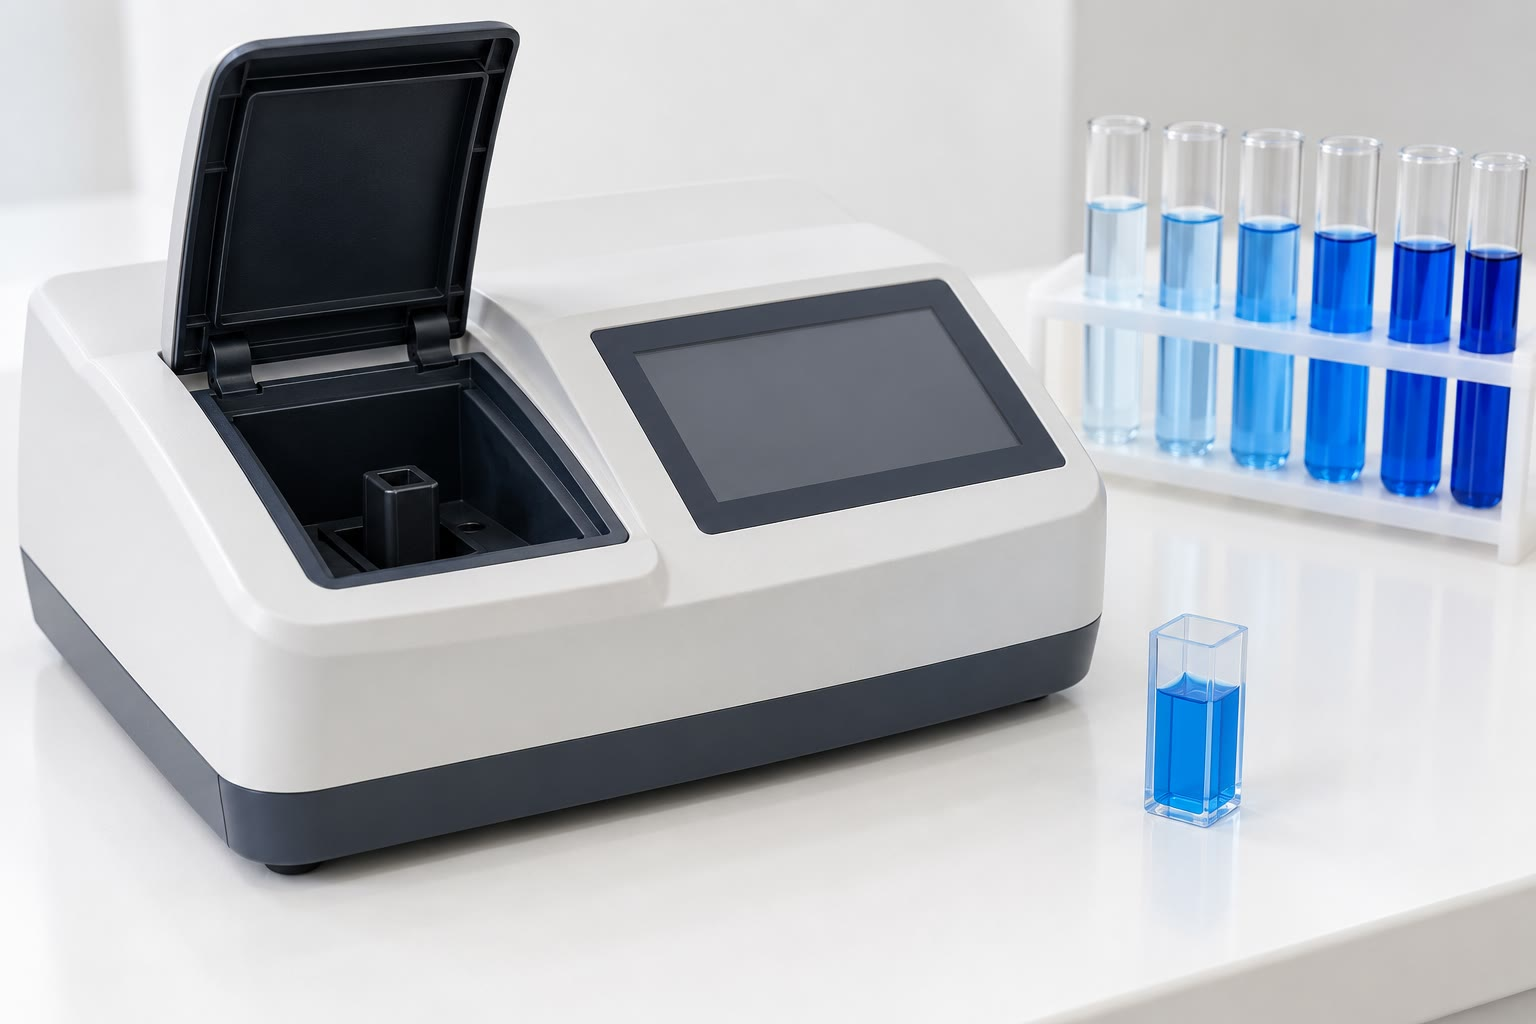
\includegraphics[width=0.5\linewidth]{images/book1/ai/g11-spectrophotometer.jpg}

{\small Sebuah spektrofotometer dan kuvet-kuvetnya yang berbentuk
persegi.}
\end{omfigure}

\section{Hukum Beer--Lambert}

\begin{definition}[Koefisien absorpsi molar]\label{def:g11:absorbance:epsilon}
Yang disebut \emph{koefisien absorpsi molar}\index{koefisien absorpsi molar}
$\varepsilon$ sebuah spesies terlarut, pada panjang gelombang tertentu,
mengukur seberapa kuat satu \omterm{def:g10:the-mole:amount}{mol} spesies itu menyerap cahaya; koefisien
ini bergantung pada spesiesnya, \omterm{def:g6:solutions-and-solubility:solute}{pelarutnya}, dan panjang gelombangnya,
dan dinyatakan dalam \si{L/(mol.cm)}.
\end{definition}

\begin{proposition}[Hukum Beer--Lambert]\label{prop:g11:absorbance:beer-lambert}
Untuk larutan encer yang hanya mengandung satu spesies penyerap, dengan
\omterm{def:g10:concentration-and-dilution:molar-concentration}{konsentrasi molar} $c$, di dalam kuvet setebal $\ell$, \omterm{def:g11:absorbance:absorbance}{absorbans} pada
panjang gelombang tertentu adalah
\[
  A = \varepsilon\, \ell\, c .
\]
\omterm{def:g11:absorbance:absorbance}{Absorbans} sebanding dengan konsentrasi.
\end{proposition}

\begin{proof}
Di sini diterima tanpa bukti; hukum ini diturunkan di salah satu buku
universitas.
\end{proof}


\begin{remark}[Dengan konsentrasi massa]\label{rem:g11:absorbance:mass}
% ledger: abs:E133, mw:E133
Karena $c = C_m / M$, hukum itu dapat pula ditulis $A = a\, \ell\, C_m$,
dengan $a = \varepsilon / M$ dalam \si{L/(g.cm)}. Spesifikasi zat warna
makanan mencantumkan $a$: untuk zat warna biru E133 pada \qty{629}{nm},
$a =
\qty{164}{L/(g.cm)}$, dan dengan \omterm{def:g10:the-mole:molar-mass}{massa molarnya} \qty{792.9}{g/mol},
$\varepsilon = 164 \times 792.9 = \qty{1.30e5}{L/(mol.cm)}$. Larutan
yang hanya mengandung \qty{5.0}{mg/L} zat warna itu, di dalam kuvet
\qty{1}{cm}, sudah menunjukkan
$A = 164 \times 1 \times 0.0050 = 0.82$.
\end{remark}

\begin{remark}[Hanya untuk larutan encer]\label{rem:g11:absorbance:dilute}
Kesebandingan itu hanya berlaku untuk larutan encer, dalam praktik untuk
\omterm{def:g11:absorbance:absorbance}{absorbans} di bawah sekitar 1 sampai 1.5 pada alat biasa. Larutan yang
terlalu pekat diencerkan dengan faktor yang diketahui sebelum diukur.
\end{remark}

\section{Mengukur konsentrasi}

\begin{definition}[Garis kalibrasi]\label{def:g11:absorbance:calibration-line}
Yang disebut \emph{garis kalibrasi}\index{garis kalibrasi} adalah grafik
\omterm{def:g11:absorbance:absorbance}{absorbans} serangkaian \omterm{def:g10:concentration-and-dilution:standard}{larutan standar} dari satu spesies, yang diukur
pada panjang gelombang yang sama di dalam kuvet yang sama, terhadap
konsentrasinya. Jika hukum Beer--Lambert berlaku, grafik itu berupa
garis lurus yang melalui titik asal.
\end{definition}

\begin{method}[Mengukur konsentrasi dengan garis kalibrasi]\label{met:g11:absorbance:calibration}
\begin{enumerate}
  \item Rekamlah \omterm{def:g11:absorbance:spectrum}{spektrum serapan} spesies itu dan pilihlah panjang
        gelombang $\lambda_{\max}$, tempat \omterm{def:g11:absorbance:absorbance}{absorbansnya} paling besar dan
        paling sedikit berubah oleh sedikit kesalahan panjang gelombang.
  \item Nolkan alat dengan blanko.
  \item Siapkan larutan-larutan standar dengan mengencerkan \omterm{def:g10:concentration-and-dilution:dilution}{larutan
        induk}, lalu ukur \omterm{def:g11:absorbance:absorbance}{absorbansnya}.
  \item Gambarlah $A$ terhadap konsentrasi, lalu tariklah garis lurus
        melalui titik asal yang paling dekat dengan titik-titik itu.
  \item Ukurlah larutan yang tidak diketahui, diencerkan jika perlu agar
        \omterm{def:g11:absorbance:absorbance}{absorbansnya} berada di antara \omterm{def:g11:absorbance:absorbance}{absorbans} larutan-larutan standar,
        lalu bacalah konsentrasinya pada garis itu (atau bagilah $A$
        dengan kemiringannya); kalikan dengan \omterm{def:g10:concentration-and-dilution:dilution}{faktor pengencerannya}.
\end{enumerate}
\end{method}

\begin{omfigure}
\begin{tikzpicture}
\begin{axis}[width=0.72\linewidth, height=6cm, xmin=0, xmax=5.6,
    ymin=0, ymax=0.95, xlabel={konsentrasi E133 (\si{mg/L})},
    ylabel={absorbans pada \qty{629}{nm}}, axis lines*=left, ymajorgrids,
    xmajorgrids, grid style={gray!20}, tick label style={font=\small},
    label style={font=\small}]
  % ledger: abs:E133 (points synthetic: exact values + fixed offsets)
  \addplot[only marks, mark=*, mark size=2.2pt, omDef] table[x=C, y=A]
    {figdata/out/grade-11-absorbance-b.dat};
  \addplot[thick, omProp, domain=0:5.5] {0.164*x};
  \addplot[dashed, black!60] coordinates {(0,0.590) (3.6,0.590) (3.6,0)};
  \node[font=\small, anchor=south west] at (axis cs:0.1,0.6) {tak diketahui: $A = 0.590$};
  \node[font=\small, anchor=west] at (axis cs:3.65,0.22) {\qty{3.6}{mg/L}};
\end{axis}
\end{tikzpicture}

{\small \omterm{def:g11:absorbance:calibration-line}{Garis kalibrasi} zat warna biru: lima \omterm{def:g10:concentration-and-dilution:standard}{larutan standar} (titik-titik)
dan garis yang melalui titik asal, dengan kemiringan \qty{0.164}{L/mg}.
Larutan tak diketahui yang menunjukkan $A = 0.590$ memiliki konsentrasi
$0.590 / 0.164 =
\qty{3.6}{mg/L}$.}
\end{omfigure}

\begin{example}[Lima larutan standar]\label{ex:g11:absorbance:standards}
\omterm{def:g10:concentration-and-dilution:dilution}{Larutan induk} zat warna biru \qty{100}{mg/L} diencerkan untuk memperoleh
\qty{100.0}{mL} setiap \omterm{def:g10:concentration-and-dilution:standard}{larutan standar}: untuk \qty{2.0}{mg/L}, \omterm{def:g10:concentration-and-dilution:dilution}{faktor
pengencerannya} 50, jadi \qty{2.0}{mL} \omterm{def:g10:concentration-and-dilution:dilution}{larutan induk} dicukupkan sampai
\qty{100.0}{mL}. Kelima \omterm{def:g10:concentration-and-dilution:standard}{larutan standar}, dari 1 sampai \qty{5}{mg/L},
menunjukkan 0.168, 0.325, 0.494, 0.652, dan 0.823: selisihnya hanya
beberapa perseribu dari $0.164 \times C$, garis pada gambar itu.
\end{example}

\section{Latihan}

\begin{exercise}[$\star$]\label{exo:g11:absorbance:1}
Sebuah larutan terutama menyerap cahaya jingga. Warna apa yang tampak?
Dan larutan yang terutama menyerap cahaya ungu?
\end{exercise}

\begin{exercise}[$\star$]\label{exo:g11:absorbance:2}
Dengan roda warna, sebutkan warna yang terutama diserap sebuah larutan
hijau, dan rentang panjang gelombang warna itu.
\end{exercise}

\begin{exercise}[$\star$]\label{exo:g11:absorbance:3}
Bacalah pada spektrum-spektrum serapan panjang gelombang $\lambda_{\max}$
setiap zat warna dan \omterm{def:g11:absorbance:absorbance}{absorbansnya} di situ.
\end{exercise}

\begin{exercise}[$\star$]\label{exo:g11:absorbance:4}
Larutan zat warna \qty{2.0}{mg/L} menunjukkan $A = 0.30$. Berapa
\omterm{def:g11:absorbance:absorbance}{absorbans} larutan zat warna yang sama \qty{6.0}{mg/L} di dalam kuvet yang
sama, pada panjang gelombang yang sama? Dan pada \qty{1.0}{mg/L}?
\end{exercise}

\begin{exercise}[$\star$]\label{exo:g11:absorbance:5}
Apa itu blanko pada spektrofotometer, dan mengapa alat itu dinolkan
dengannya?
\end{exercise}

\begin{exercise}[$\star\star$]\label{exo:g11:absorbance:6}
Dengan \omterm{def:g11:absorbance:calibration-line}{garis kalibrasi} zat warna biru, tentukan konsentrasi larutan yang
menunjukkan $A = 0.41$.
\end{exercise}

\begin{exercise}[$\star\star$]\label{exo:g11:absorbance:7}
Untuk mengukur zat warna biru, mengapa spektrofotometer diatur pada
\qty{629}{nm} dan bukan pada \qty{550}{nm}? Berikan dua alasan.
\end{exercise}

\begin{exercise}[$\star\star$]\label{exo:g11:absorbance:8}
Sebuah minuman yang belum diencerkan menunjukkan $A = 2.4$ pada
\qty{629}{nm}, terlalu tinggi untuk dipercaya. Minuman itu diencerkan
lima kali lalu menunjukkan $A = 0.48$. Tentukan konsentrasi zat warna
biru dalam minuman itu.
\end{exercise}

\begin{exercise}[$\star\star$]\label{exo:g11:absorbance:9}
% ledger: mw:E102, abs:E102
Larutan tartrazin \qty{15.0}{mg/L} menunjukkan $A = 0.795$ pada
\qty{427}{nm} di dalam kuvet \qty{1.00}{cm}. Hitung absorptivitasnya $a$
dalam \si{L/(g.cm)}, lalu \omterm{def:g11:absorbance:epsilon}{koefisien absorpsi molarnya} (\omterm{def:g10:the-mole:molar-mass}{massa molar}
\qty{534.4}{g/mol}).
\end{exercise}

\begin{exercise}[$\star\star$]\label{exo:g11:absorbance:10}
Lihatlah spektrum kedua zat warna. Di atas panjang gelombang berapa zat
warna kuning hampir tidak menyerap apa pun? Mengapa zat warna biru dapat
diukur pada \qty{629}{nm} bahkan dalam minuman hijau yang juga
mengandung zat warna kuning?
\end{exercise}

\begin{exercise}[$\star\star$]\label{exo:g11:absorbance:11}
Larutan yang sama diukur di dalam kuvet setebal \qty{2.0}{cm} alih-alih
\qty{1.0}{cm}. Bagaimana \omterm{def:g11:absorbance:absorbance}{absorbansnya} berubah? Mengapa?
\end{exercise}

\begin{exercise}[$\star\star\star$]\label{exo:g11:absorbance:12}
\omterm{def:g10:concentration-and-dilution:standard}{Larutan standar} zat warna biru 5, 10, 20, dan \qty{40}{mg/L} menunjukkan
0.82, 1.62, 2.30, dan 2.70. Hitung $A / C$ untuk masing-masing. Apa yang
kamu perhatikan? \omterm{def:g10:concentration-and-dilution:standard}{Larutan standar} mana yang boleh dipakai untuk \omterm{def:g11:absorbance:calibration-line}{garis
kalibrasi}, dan apa yang harus dilakukan dengan larutan tak diketahui
yang menunjukkan $2.5$?
\end{exercise}

\begin{exercise}[$\star\star\star$]\label{exo:g11:absorbance:13}
Sebuah minuman hijau mengandung zat warna biru dan zat warna kuning. Di
dalam kuvet \qty{1.00}{cm} minuman itu menunjukkan $A = 0.574$ pada
\qty{629}{nm} dan $A = 0.53$ pada \qty{427}{nm}. Pada \qty{427}{nm} zat
warna biru hampir tidak menyerap apa pun, dan pada \qty{629}{nm} zat
warna kuning tidak menyerap apa pun. Tentukan \omterm{def:g10:concentration-and-dilution:mass-concentration}{konsentrasi massa} kedua
zat warna itu (pakailah $a = \qty{164}{L/(g.cm)}$ dan
$a = \qty{53.0}{L/(g.cm)}$).
\end{exercise}

\begin{exercise}[$\star\star\star$]\label{exo:g11:absorbance:14}
Seorang siswa lupa memakai blanko dan menolkan alat dengan kuvet
kosong. Akibatnya setiap pembacaan \num{0.040} terlalu tinggi. Larutan
tak diketahui menunjukkan $0.368$, dan ia membaginya dengan kemiringan
$0.164$ dari \omterm{def:g11:absorbance:calibration-line}{garis kalibrasi} yang benar. Berapa konsentrasi yang
diperolehnya? Berapa konsentrasi yang sebenarnya? Berapa persen
kesalahannya?
\end{exercise}

\begin{exercise}[$\star\star\star$]\label{exo:g11:absorbance:15}
% ledger: adi:E102
Asupan harian yang dapat diterima untuk tartrazin adalah \qty{10}{mg}
per kilogram massa tubuh. Sebuah minuman mengandung \qty{20}{mg/L}
tartrazin. Berapa volume minuman yang akan membawa seorang dewasa
seberat \qty{60}{kg} mencapai asupan ini dalam sehari? Apakah itu risiko
yang realistis?
\end{exercise}

\section{Soal: Biru Minuman Olahraga}


\begin{problem}[{Soal akhir pekan --- berapa botol minuman olahraga biru
yang harus diminum seorang anak untuk mencapai batas harian yang aman
untuk zat warnanya?}]
\label{pb:g11:absorbance:1}
% ledger: lmax:E133, abs:E133, mw:E133, adi:E133
Sebuah laboratorium pangan memeriksa zat warna biru E133 dalam minuman
olahraga yang dijual dalam botol \qty{500}{mL}. Spesifikasi zat warna itu
mencantumkan \omterm{def:g10:the-mole:molar-mass}{massa molarnya}, \qty{792.9}{g/mol}, dan asupan harian yang
dapat diterima: \qty{6}{mg} per kilogram massa tubuh per hari, jumlah
yang dapat dimakan setiap hari seumur hidup tanpa risiko yang berarti.

\medskip
\noindent\textbf{Bagian I --- Warna dan spektrum.}
\begin{enumerate}
  \item Minuman itu tampak biru. Dengan roda warna, cahaya warna apa
        yang paling banyak diserapnya?
  \item Bacalah panjang gelombang $\lambda_{\max}$ zat warna itu pada
        spektrumnya.
  \item Mengapa \omterm{def:g11:absorbance:absorbance}{absorbans} zat warna itu hampir nol pada \qty{450}{nm}?
        Apakah hal itu sesuai dengan warnanya?
  \item Pada panjang gelombang berapa pengukuran harus dilakukan?
\end{enumerate}

\medskip
\noindent\textbf{Bagian II --- \omterm{def:g11:absorbance:calibration-line}{Garis kalibrasi}.}
\begin{enumerate}[resume]
  \item Sebanyak \qty{50.0}{mg} zat warna murni dilarutkan menjadi
        \qty{500.0}{mL} \omterm{def:g10:concentration-and-dilution:dilution}{larutan induk}. Hitung \omterm{def:g10:concentration-and-dilution:mass-concentration}{konsentrasi massanya} dalam
        \si{mg/L}.
  \item \omterm{def:g10:concentration-and-dilution:standard}{Larutan standar} 1.0, 2.0, 3.0, 4.0, dan \qty{5.0}{mg/L} dibuat,
        masing-masing \qty{100.0}{mL}. Berapa volume \omterm{def:g10:concentration-and-dilution:dilution}{larutan induk} yang
        diperlukan untuk \omterm{def:g10:concentration-and-dilution:standard}{larutan standar} \qty{3.0}{mg/L}? Dengan alat
        gelas apa?
  \item Larutan-larutan standar itu menunjukkan 0.168, 0.325, 0.494,
        0.652, dan 0.823. Hitung $A / C$ untuk masing-masing, lalu
        tunjukkan bahwa titik-titiknya terletak dekat garis yang melalui
        titik asal dengan kemiringan sekitar \qty{0.164}{L/mg}.
  \item Mengapa garis itu harus melalui titik asal?
  \item Simpulkan absorptivitas $a$ zat warna itu dalam \si{L/(g.cm)}
        (kuvet \qty{1.00}{cm}), lalu \omterm{def:g11:absorbance:epsilon}{koefisien absorpsi molarnya}.
\end{enumerate}

\medskip
\noindent\textbf{Bagian III --- Minumannya.}
\begin{enumerate}[resume]
  \item Sebanyak \qty{25.0}{mL} minuman dicukupkan sampai \qty{50.0}{mL}
        dengan air. Berapa \omterm{def:g10:concentration-and-dilution:dilution}{faktor pengencerannya}?
  \item Minuman yang telah diencerkan menunjukkan $A = 0.590$. Tentukan
        konsentrasi zat warnanya.
  \item Simpulkan konsentrasi zat warna dalam minuman itu sendiri.
  \item Berapa \omterm{def:g11:absorbance:absorbance}{absorbans} minuman yang belum diencerkan? Mengapa minuman
        itu diencerkan?
  \item Hitung massa zat warna dalam satu botol.
  \item Hitung \omterm{def:g10:the-mole:amount}{jumlah zat} warna, dalam \omterm{def:g10:the-mole:amount}{mol}, dalam satu botol.
\end{enumerate}

\medskip
\noindent\textbf{Bagian IV --- Asupan harian yang dapat diterima.}
\begin{enumerate}[resume]
  \item Berapa massa zat warna itu yang boleh dikonsumsi setiap hari oleh
        seorang anak seberat \qty{30}{kg}?
  \item Berapa botol yang harus diminum anak itu dalam sehari untuk
        mencapainya?
  \item Berapa volume minuman itu? Berikan tanggapan.
  \item Pertanyaan yang sama untuk orang dewasa seberat \qty{70}{kg}.
  \item Nyatakan jawaban akhirnya: berapa botol \qty{500}{mL} yang harus
        diminum seorang anak seberat \qty{30}{kg} dalam sehari untuk
        mencapai asupan harian yang dapat diterima untuk zat warna itu?
\end{enumerate}
\end{problem}
